We report ranks averaged over ten complete generation-and-evaluation runs.
Main-text heatmaps display integer ranks induced by the unrounded mean ranks;
the supplement reports means and standard errors. Results characterize the
bounded, single-turn tasks studied here and should not be interpreted as a
general ordering for tool-using or multi-turn agents.

\subsection{Rankings Depend on Usage Mode}

\begin{figure*}[t]
\centering
\begin{minipage}{0.495\textwidth}
  \centering
  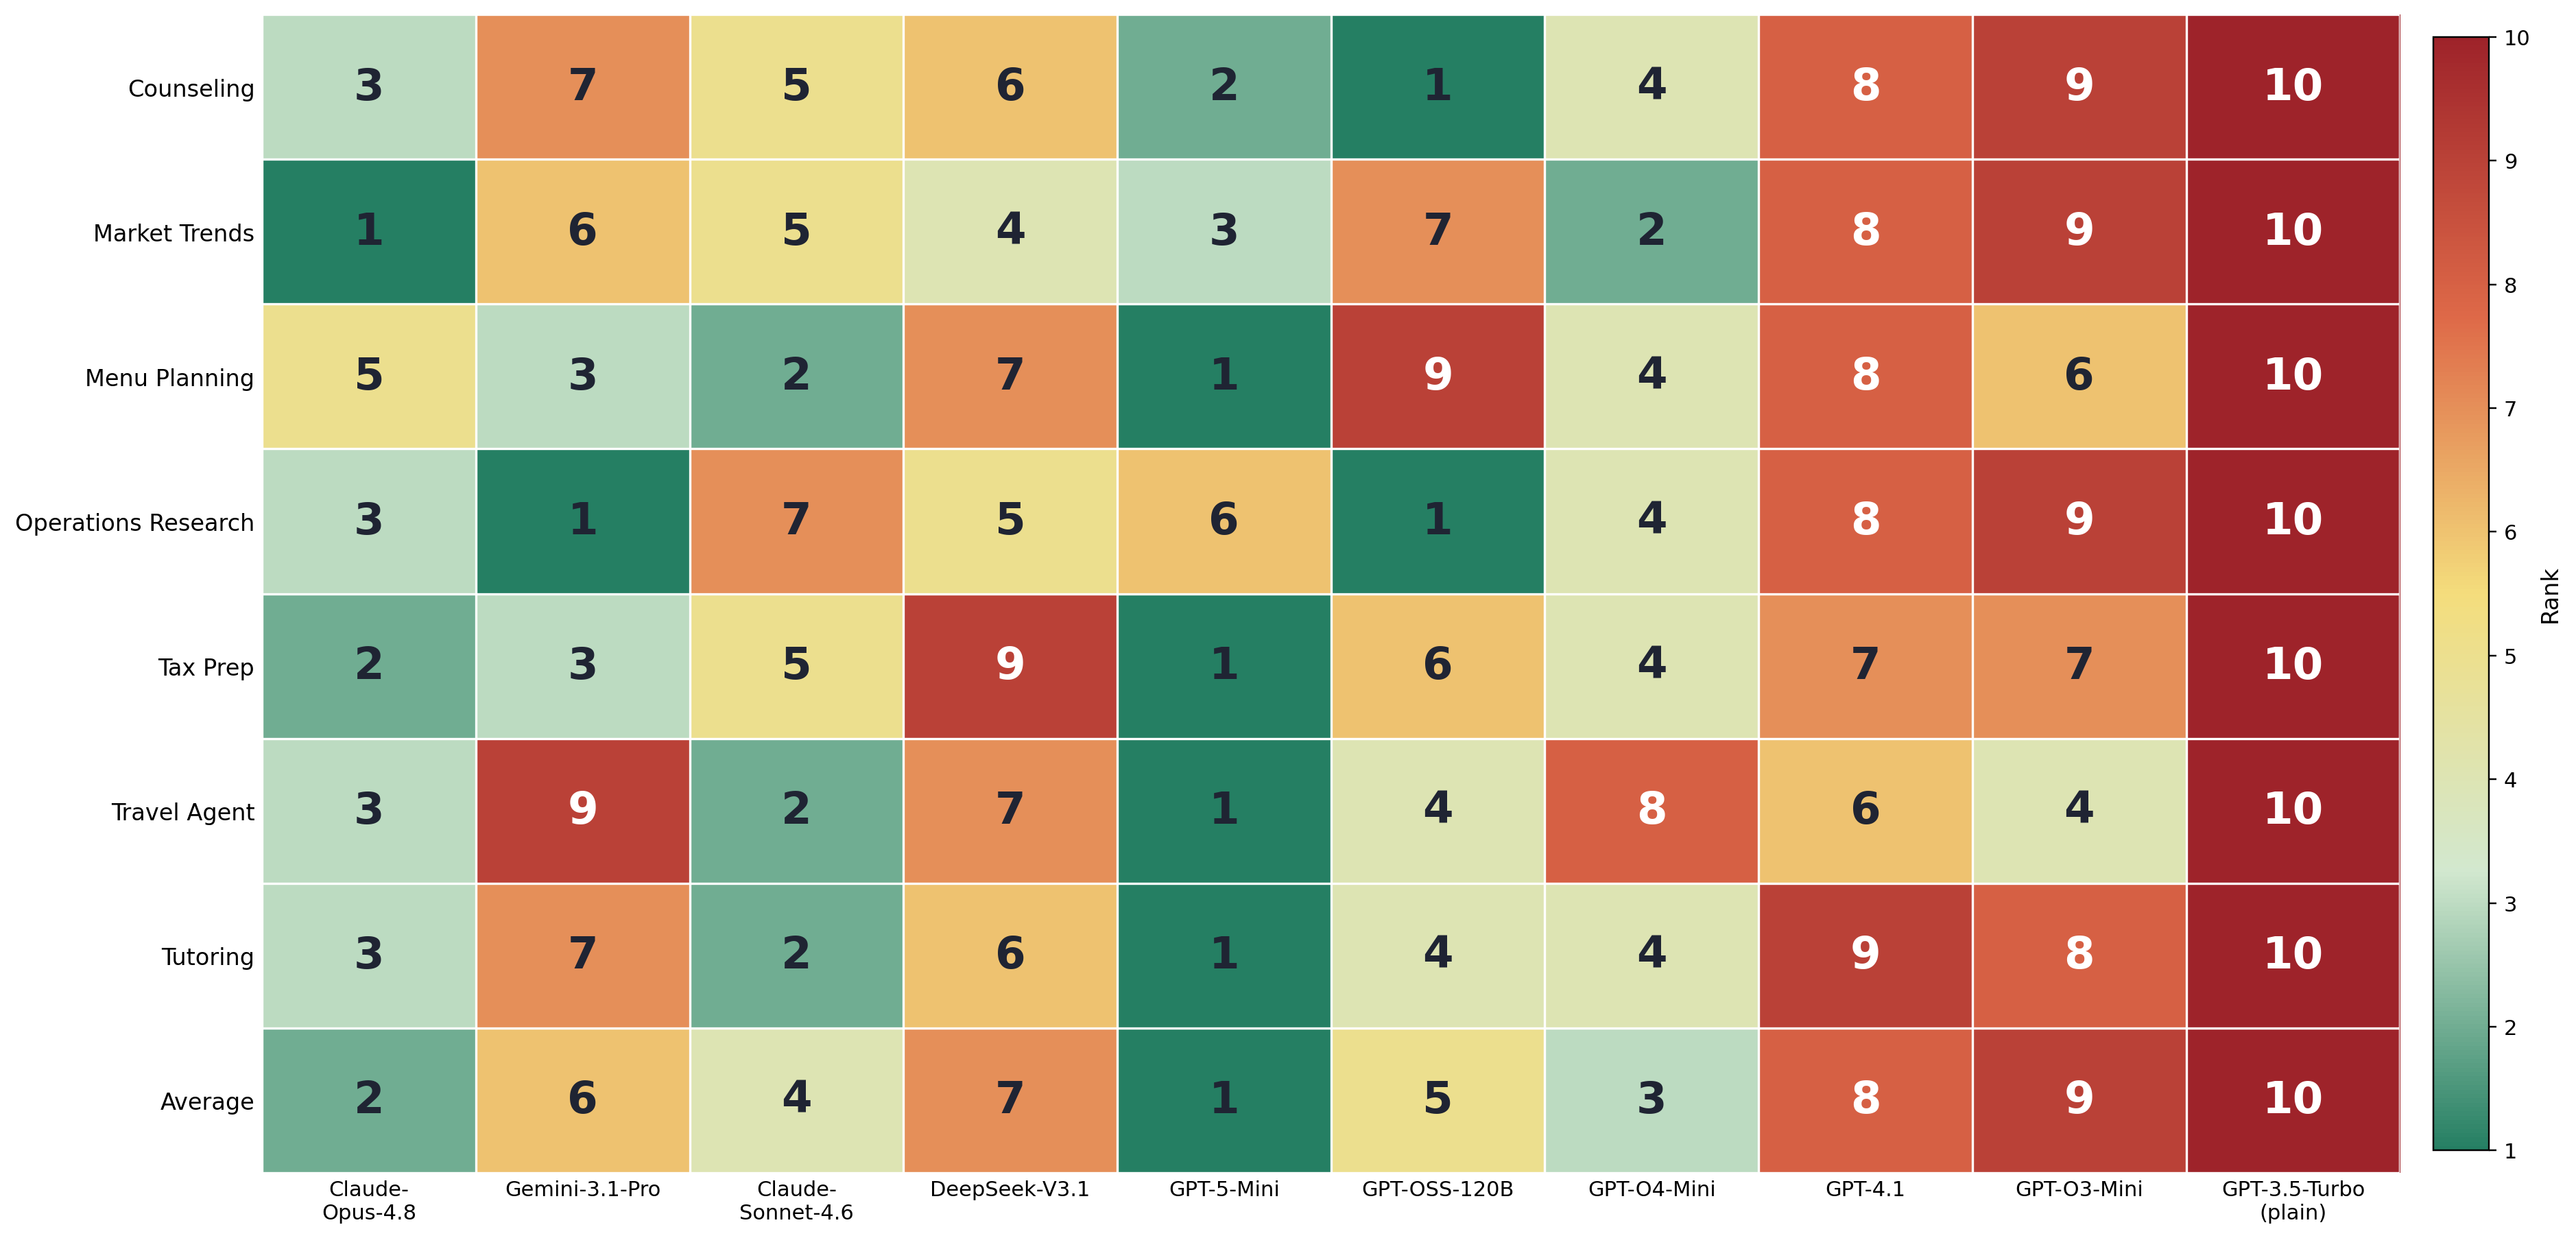
\includegraphics[width=\linewidth]{figures/figure2a_automation_heatmap.png}
  \small (a) Automation
\end{minipage}\hfill
\begin{minipage}{0.495\textwidth}
  \centering
  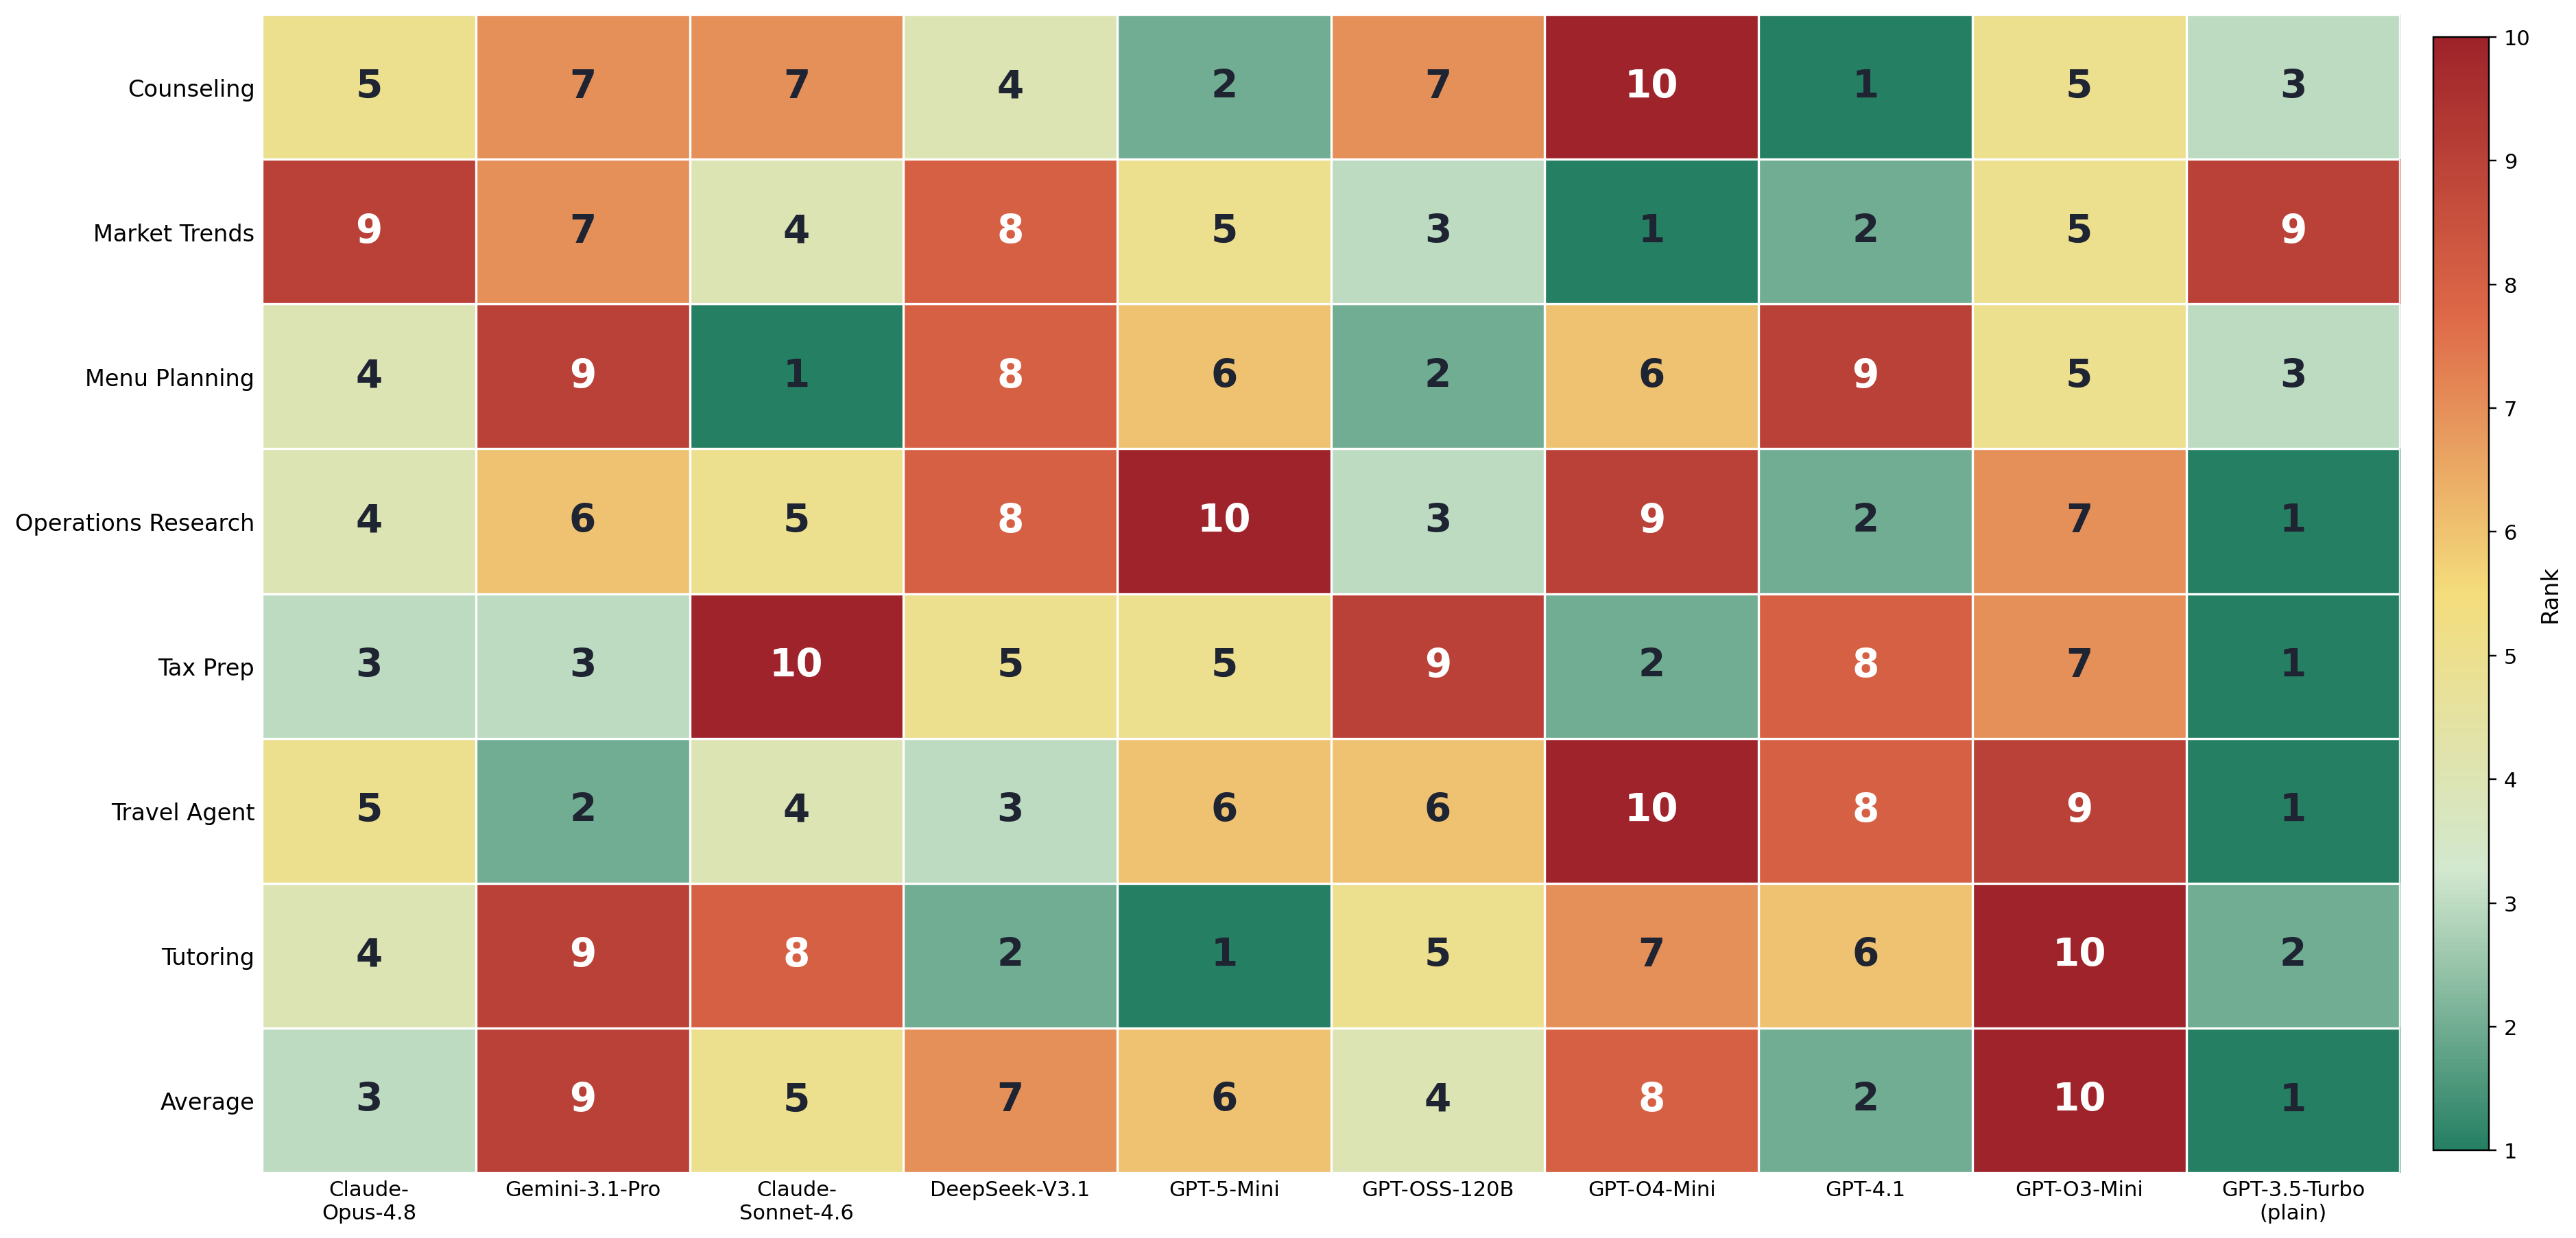
\includegraphics[width=\linewidth]{figures/figure1_augmentation_heatmap.png}
  \small (b) Augmentation
\end{minipage}
\caption{\textbf{Task-level rankings by usage mode.} Lower ranks are better.
Automation compares direct task outputs. Augmentation compares outputs from a
fixed worker conditioned on each assistant's guidance and includes the
unaided worker (plain). Rankings are computed from unrounded mean ranks across
ten runs; uncertainty estimates are in the supplement.}
\label{fig:mode-heatmaps}
\end{figure*}

Automation rankings are comparatively concentrated
(Figure~\ref{fig:mode-heatmaps}a). GPT-5-Mini has the best average rank and
wins four tasks; Claude-Opus-4.8 ranks second on average. GPT-3.5-Turbo ranks
last, consistent with the direct-solver role placing the full burden of
constraint tracking, reasoning, and deliverable production on one model.

Augmentation produces a different profile
(Figure~\ref{fig:mode-heatmaps}b). No assistant dominates across tasks:
GPT-4.1 leads counseling, GPT-O4-Mini leads market-trends analysis, and
GPT-5-Mini leads menu planning and tutoring. More importantly, the unaided
worker ranks first on operations research, tax preparation, and travel
planning. Thus, adding guidance is not automatically beneficial, even when
the assistant is a stronger standalone model than the worker.

\subsection{Automation Is an Incomplete Proxy for Assistance}

For each model, task, and mode, we average rank across runs. We compute
Spearman correlation between the automation and augmentation rank vectors
within each task, excluding the unaided worker, and repeat the comparison
after averaging each model's ranks across tasks.

\begin{figure}[t]
    \centering
    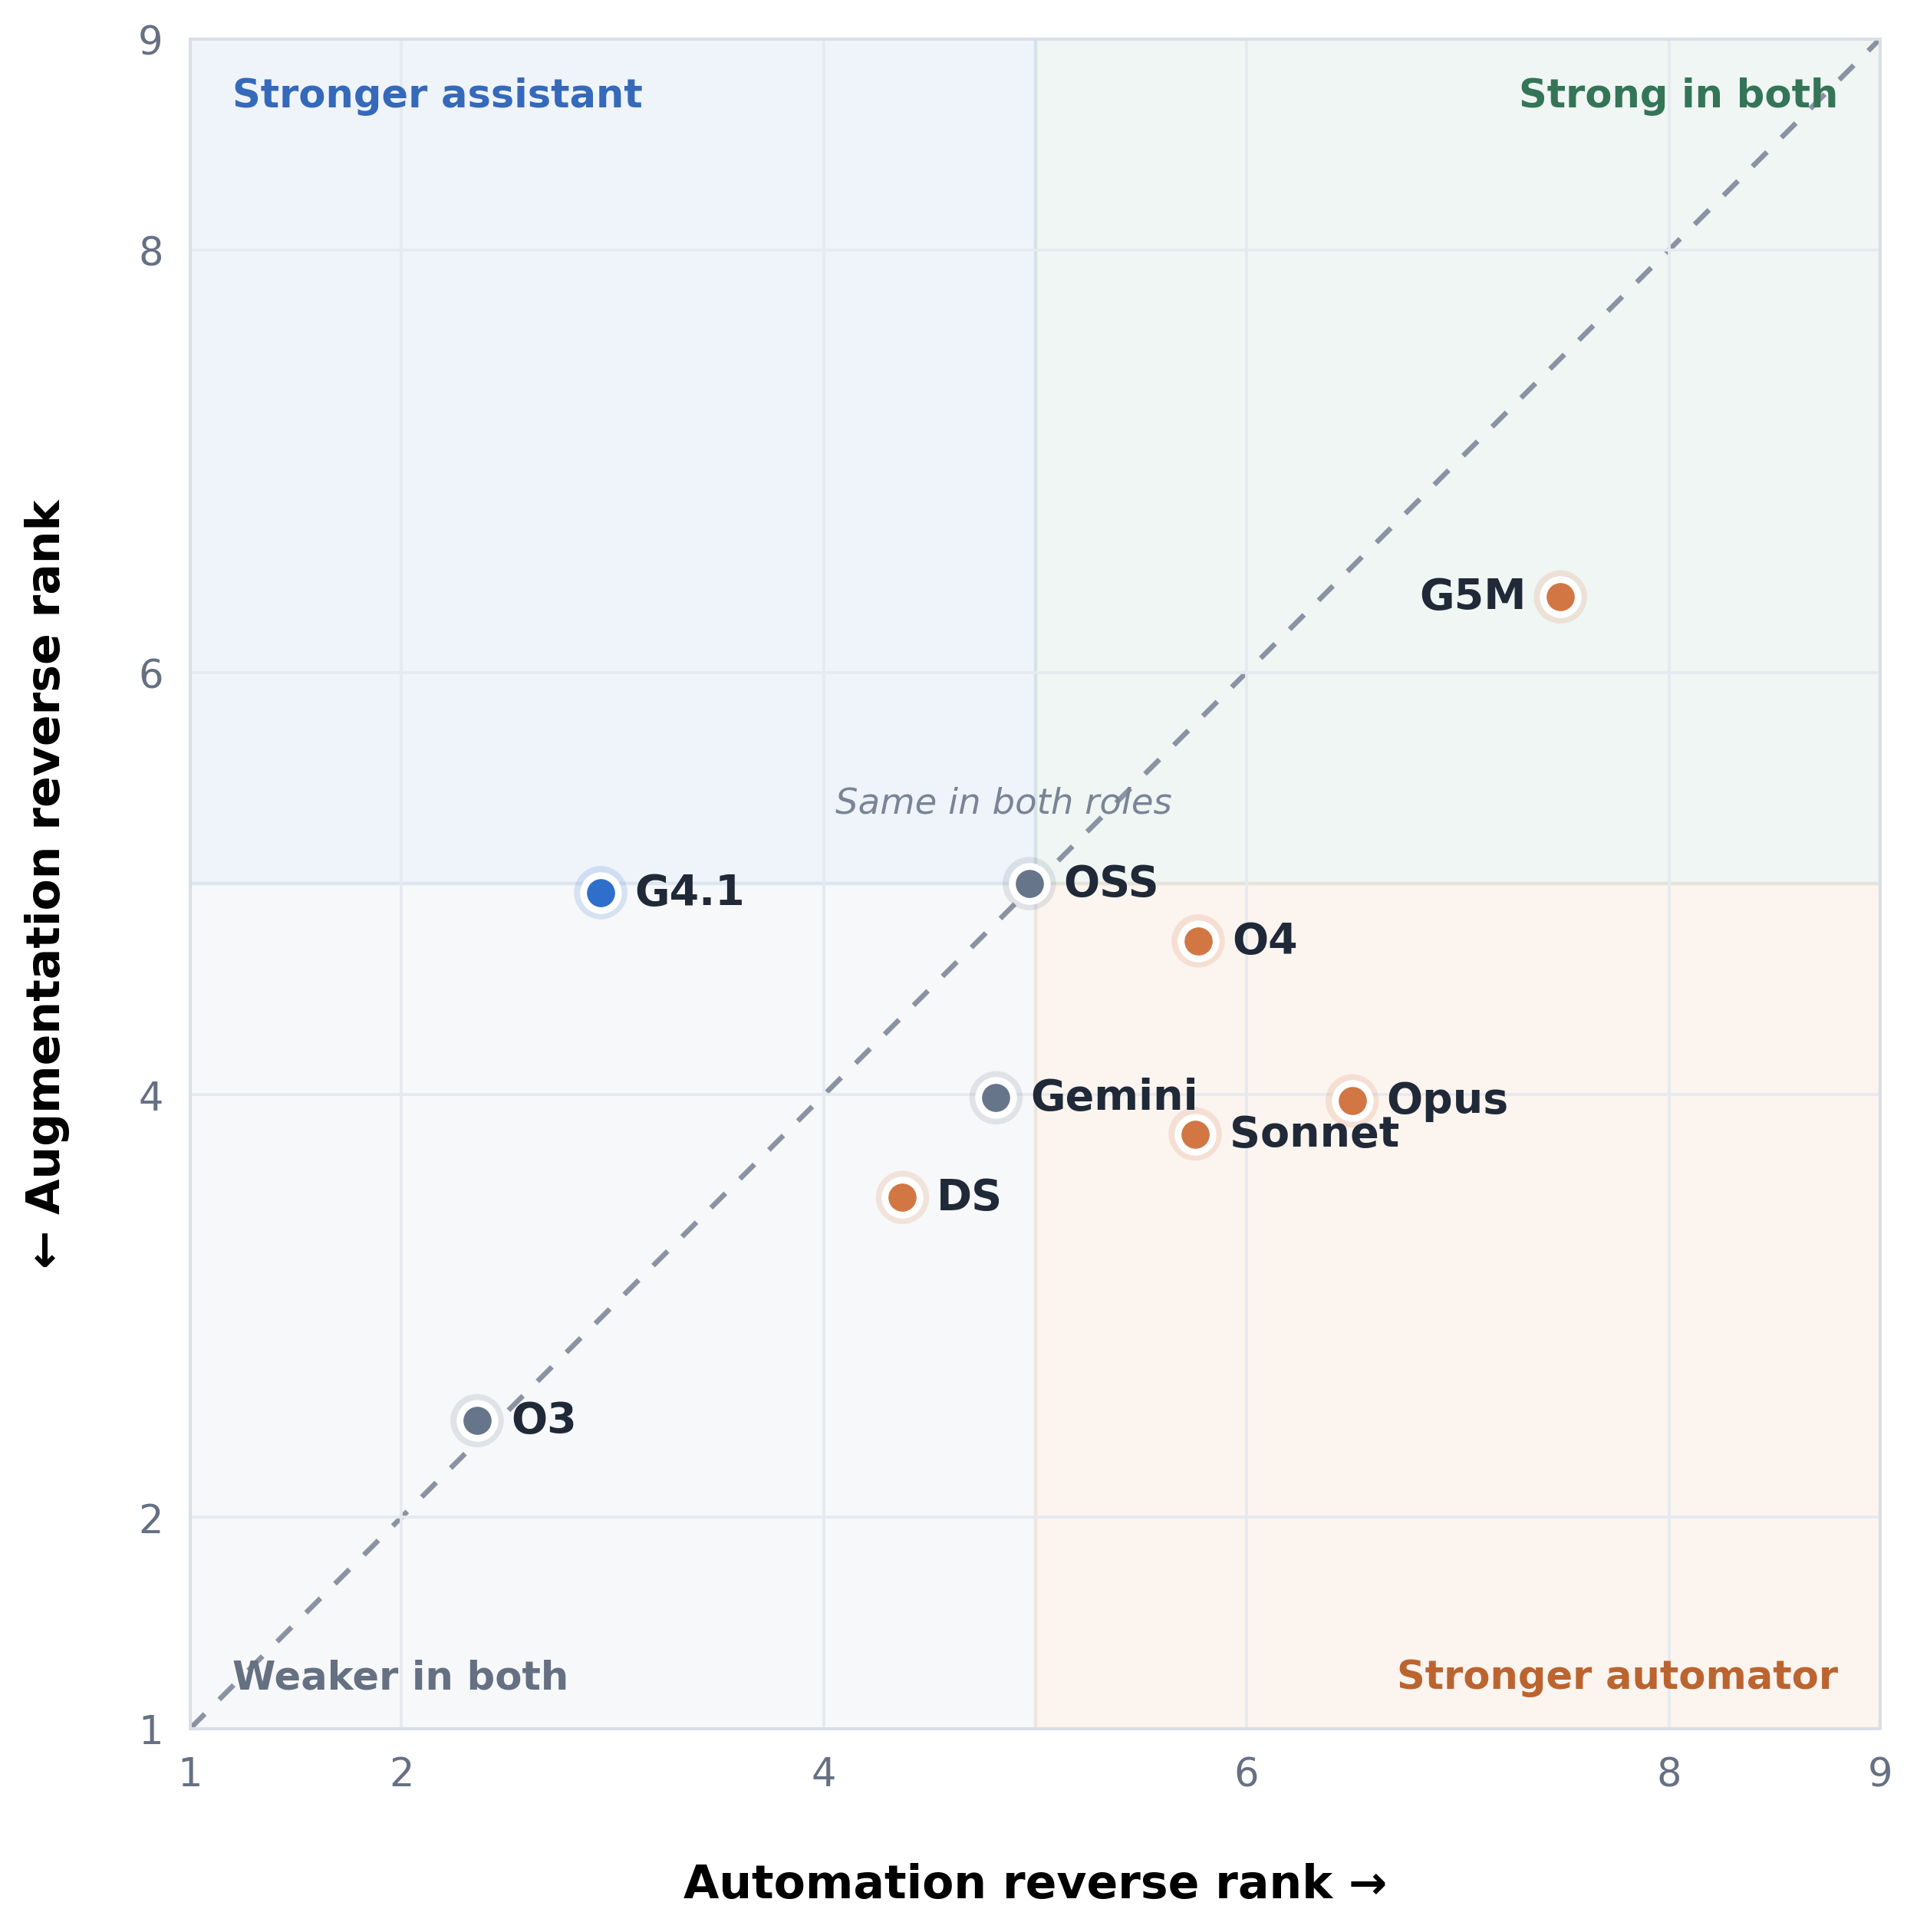
\includegraphics[width=0.82\linewidth]{figures/figure2b_role_swap_scatter_white.png}
    \caption{\textbf{Model-level role comparison.} Each point is one focal
    model's average reverse rank across seven tasks and ten runs; higher is
    better. The unaided worker is excluded.}
    \label{fig:role-swap-scatter}
\end{figure}

The model-level correlation is moderate
($\rho=0.48$, two-sided $p=0.187$; Figure~\ref{fig:role-swap-scatter}).
Automation therefore contains some information about assistant quality but
does not recover the same ordering. Task-level correlations vary sharply:
tax preparation has the strongest association ($\rho=0.85$), followed by menu
planning ($0.64$) and tutoring ($0.50$); counseling ($0.25$), operations
research ($0.17$), and market trends ($0.10$) are weakly associated, while
travel planning is essentially unrelated ($-0.04$). The complete correlation
table and significance tests are in the supplement.

The winning condition differs across modes on five of seven tasks. The plain
worker has an average augmentation rank of $3.79$; GPT-5-Mini is the only
assisted condition with a better average rank ($3.66$). This result does not
imply that assistance is generally ineffective. Rather, the value of guidance
depends on its compatibility with the task and worker, and a strong unaided
baseline can outperform guidance that adds irrelevant constraints or
misdirects execution.

Task-level reversals can be large. On market-trends analysis,
Claude-Opus-4.8 is the strongest automator (mean rank $2.05$) but one of the
weakest assistants ($8.15$). On counseling, GPT-4.1 is substantially stronger
as an assistant (mean rank $3.80$, best among assisted conditions) than as an
automator ($7.40$). These gaps persist after averaging ten runs, rather than
being driven by one stochastic generation.

\subsection{What Distinguishes Useful Guidance?}
\label{sec:analysis}

We qualitatively compare assistance texts associated with the two
highest- and two lowest-ranked outputs for each task. Higher-ranked guidance
tends to add task-specific analytical steps beyond restating the prompt,
impose a usable output structure, and preserve the worker's responsibility
for completing the requested deliverable. Lower-ranked guidance is often
generic, delegates key structural decisions back to the worker, or actively
discourages required analysis. In the operations-research task, for example,
a low-ranked assistant tells the worker not to provide specific solutions
even though the task explicitly requires two solutions and their trade-offs.
These observations are descriptive rather than causal, but they offer a
mechanism for why no assistance can outperform poorly calibrated assistance.
The coded examples and full assistance excerpts are provided in the
supplement.
